\documentclass[a4paper,11pt,article,oneside]{memoir}

% Sproget sættes til dansk og orddeling indlæses
\usepackage[utf8]{inputenc}
\usepackage[T1]{fontenc}
\usepackage[english]{babel}

% Matematiske symboler og fede tegn i ligninger
\usepackage{amsmath, amssymb, bm, mathtools}

% Tabeller og søjler
\usepackage{array, booktabs, dcolumn}
\newcolumntype{d}[1]{D{,}{,}{#1}} % Justering under komma

% Figurer
\usepackage{graphicx, placeins, subfig}
\captionsetup{font=small,labelfont=bf}
\graphicspath{{../}}
\usepackage{url}

%Colors
\usepackage{xcolor}
\definecolor{nicered}{rgb}{.647,.129,.149}
\newcommand{\pyt}[1]{\textbf{\textcolor{olive}{#1}}}
\newcommand{\dt}[1]{\textcolor{teal}{#1}}
\newcommand{\func}[1]{\textbf{\textcolor{blue}{#1}}}
\newcommand{\va}[1]{\textcolor{nicered}{#1}}
\newcommand{\red}[1]{\textcolor{red}{#1}}

\begin{document}
\author{S\o ren Frimann}
\title{Gaussian Processes for non-linear regression and prediction problems}
\date{\today}
\maketitle

\chapter{Introduction}
Gathering and interpretation of data is a key aspect in science, and creating good models is often a crucial point in the analysis -- this however often turns out to be a very tricky problem. The classical approach to modelling is to choose a parametric model and run some kind of optimizer to maximize the likelihood of the model. For complicated models that might suffer from a large amount of narrow local minima more sophisticated (and time consuming) approaches such as \emph{Markov Chain Monte Carlo} might be chosen.

\emph{Gaussian Processes Regression} (GPR) is a paradigm in \emph{Supervised Learning}, that makes you able to solve non-linear regression and prediction problems without having to resort to parametric models which are not very flexible with regard to the data (the data has to be well represented by the parametric model), and might be difficult to get to converge. \fref{fig:regression} shows a typical example of a regression problem that can be solved by GPR. Given a set of noisy observations, $\mathcal{D} = (\mathbf{x},\mathbf{y})$, assumed to be drawn from an underlying \emph{latent function}, $f(x)$, we wish to estimate the function value, at all other inputs, $\mathbf{x}_\star$. The classical approach would be to try a number of different parametric models, choosing the one that gives the highest probability (I avoid saying likelihood since more complex models will usually be able to fit the data better, but not generally be the best choice). GPR is another approach where one does not assume the data to follow a specific parametric model, instead it enables the data to ``speak for itself'' -- as we will see later one will still have to make assumptions about the data, but these assumptions doesn't operate at the same level as the data.

\begin{figure}[htb]
\centering
\includegraphics[width=0.49\textwidth]{fig1} 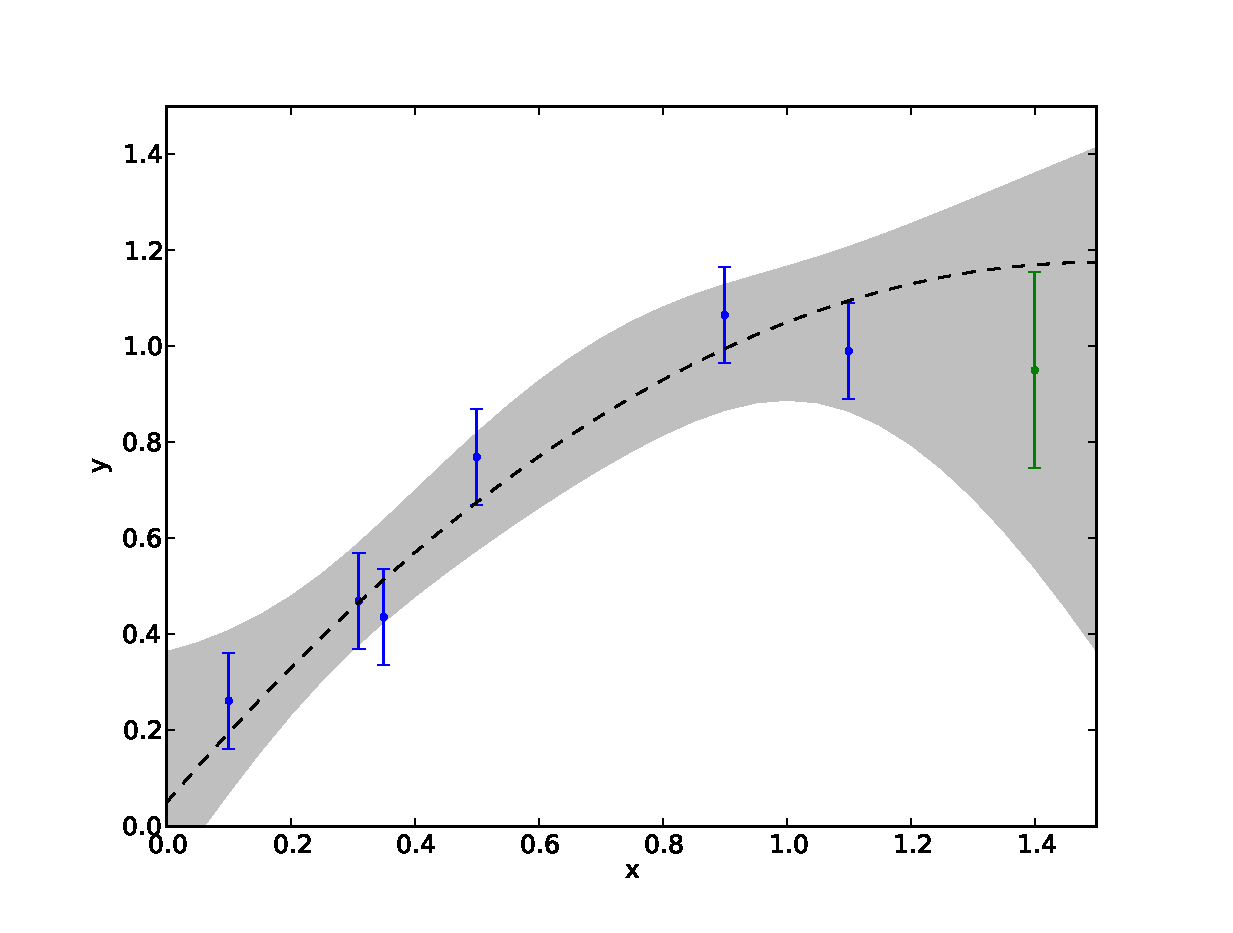
\includegraphics[width=0.49\textwidth]{fig2}
\caption{The classical regression problem. Left: Given six noisy data point we are interested in estimating the value of a seventh point at $x_\star=1.4$. Right: The solution to the problem. The shaded area show the $2\sigma$ confidence interval for the value of the underlying function, while the green point show the predicted function value and $1\sigma$ uncertainty of the underlying function at $x_\star=1.4$. The dashed line shows the actual function from which the observations were drawn in the first place.}
\label{fig:regression}
\end{figure}

The outline of the report is the follwing: In section~\ref{sec:theory} I will briefly go through the idea and theory behind \emph{Gaussian Processes} (GPs), while simultaneously touch upon the subject of \emph{Bayesian Inference}, since this is the framework in which we'll be working. In section~\ref{sec:description} I outline how to use the software I've written for the project, and describe the most essential code. In section~\ref{sec:tests} I'll test the software on synthetic data to see how well it performs, before applying it to a real-life example in section~\ref{sec:example}. In section~\ref{sec:discussion} I'll discuss and conclude on the project.

All programming for this project was done in \emph{Python}. The main purpose of this project has been to investigate and implement GPR, and I've therefore allowed myself to use some high-level routines already built into Python (or more specifically numpy and scipy). These include routines to do \emph{Cholesky Decomposition}, and drawing samples from a \emph{multivariate Gaussian Distribution}, but they also include routines to do \emph{Downhill Simplex} optimization, and for solving linear systems of equations. I chose to go with the library routines, rather than the ones developed during the course, partly due to considerations of speed, and partly due to bugs that might linger in my own code, and make implementation of the Gaussian Processes more difficult.

\chapter{Theory}
\label{sec:theory}

A multivariate Gaussian distribution is fully specified by its mean vector, $\boldsymbol{\mu}$, and covariance matrix, $\Sigma$, such that when we draw a sample from the distribution we get a vector, $\mathbf{f} \sim \mathcal{N}\left( \boldsymbol{\mu}, \Sigma \right)$. A Gaussian Process can be thought of as a continuous generalization of a multivariate Gaussian distribution. Formally:
%
\begin{quote}
\textbf{Definition:} A Gaussian Process is a collection of random variables, any finite number of which have a joint Gaussian distribution \cite{rasmussen2006}
\end{quote}
%
In manner analougous to Gaussian distributions Gaussian Processes are fully specified by a mean function, $m(x)$, and a covariance function, $k(x,x')$, so that we can draw a sample, $f(x) \sim \mathcal{GP}\left( m(x), k(x,x') \right)$ from the GP. Working with continuous variables is not feasible when doing numerical calculations, but we're saved by the \emph{marginalization property} which for multivariate Gaussians is a simple matter of dropping the variables one is not interested in \cite{wiki:gauss}. More specifically:
%
\begin{equation}
p(\mathbf{x},\mathbf{y}) = \mathcal{N}\left( \begin{bmatrix} \mathbf{a} \\ \mathbf{b} \end{bmatrix} , \begin{bmatrix} A & C \\ C^T & B \end{bmatrix} \right) \Longrightarrow p(\mathbf{x}) = \mathcal{N}\left( \mathbf{a} , A \right). \nonumber
\end{equation}
%
This property means that it doesn't matter that we only look at a finite number of points in the Gaussian Process, since marginalizing out the rest won't change it!

As mentioned above you are not free of making some assumptions about the data when doing GPR. More specifically you have to imagine that your observations, $\mathcal{D} = (\mathbf{x},\mathbf{y})$, can be drawn from a multivariate Gaussian distribution with mean, $m(\mathbf{x})$, and covariance matrix, $K$, defined as the \emph{Gram Matrix} of the covariance function, $k(x,x')$\cite{wiki:gram}. The results then ultimately depends on the choice of mean and covariance function for the GP. The mean function can be whatever function you like (often it is simply assumed to be zero), while the covariance function has to be positive semidefinite \cite[Chapter~4]{rasmussen2006}. A widely used covariance function is the \emph{Squared Exponential}:
%
\begin{equation}
k(x,x') = \sigma_f^2 \exp\left( -\frac{(x-x')^2}{2\ell^2}\right).
\label{eq:se}
\end{equation}
%
This covariance function is \emph{stationary} -- that is it only depends on the distance between $x$ and $x'$ not the actual inputs themselves -- and secures a high covariance between points lying close together, which ensures that the samples drawn from the GP will be smooth. $\sigma_f$ and $\ell$ are the so-called \emph{hyperparameters} (the set of them usually written as $\boldsymbol{\theta}$). Note that $\sigma_f$ and $\ell$ are both examples of \emph{scale parameters}, that is parameters that are naturally positive. For scale parameters we will always work with the natural logarithm of the actual paramter -- this is done to prevent problems during \emph{optimization} later on where the chosen optimizer cannot be restricted only to take on positive values. Depending on the training set at hand, different values of the hyperparameters, or different covariance functions altogether might be appropriate. Other examples of covariance functions, and their properties can be found in \cite[Chapter~4]{rasmussen2006}, but  examples are also given in sections~\ref{sec:tests} and~\ref{sec:example}.

\section{Bayesian Inference}
In the following, I will briefly go through the framework of \emph{Bayesian Inference}. This is pretty basic and covered in most elementary texts on the subject -- a good introductory text is \cite{gregory2005}. Specific information relating to Gaussian Processes is covered in \cite[Chapter~2]{rasmussen2006}, and it is from here that most of the results in this section are quoted.

When working with GPR we will generally assume that we have a set of noisy observations, $\mathbf{y}$, where each point can be described as:
%
\begin{equation}
y_i = f(x_i) + \epsilon_i. \nonumber
\end{equation}
%
$f(x)$ is the underlying latent function, and $\epsilon \sim \mathcal{N}(0,\sigma_n^2)$ is \emph{independent identically distributed} (IID) Gaussian noise with zero mean and variance $\sigma_n^2$. Using these assumptions we can calculate the \emph{likelihood} which will be given as a Gaussian distribution:
%
\begin{equation}
p(\mathbf{y}|\mathbf{x},\mathbf{f}) = \mathcal{N}(\mathbf{f},\sigma_n^2I).
\label{eq:likelihood}
\end{equation}
%
Here $\mathbf{f}$ is a vector of our best estimates for the value of the latent function, $f(x)$, at the same inputs, $\mathbf{x}$, as the targets, $\mathbf{y}$. $I$ is the Identity matrix. We also define a prior probability for $\mathbf{f}$, encoding what we believe to be known about the system beforehand. This prior is assumed to be a multivariate Gaussian:
%
\begin{equation}
p(\mathbf{f}|\boldsymbol{\theta},M_i) = \mathcal{N}(\mathbf{m},K).
\label{eq:prior}
\end{equation}
%
$K$ and $\mathbf{m}$ are the covariance matrix and mean vector, respectively constructed from the covariance and mean function of the GP. As such the prior will be conditioned on the choice of hyperparameters, $\boldsymbol{\theta}$, and model (covariance function), $M_i$. We can get the posterior distribution by using \emph{Bayes' Theorem}:
%
\begin{equation}
p(\mathbf{f}|\mathbf{y},\mathbf{x},\boldsymbol{\theta},M_i) = \frac{p(\mathbf{y}|\mathbf{x},\mathbf{f})p(\mathbf{f}|\boldsymbol{\theta},M_i)}{p(\mathbf{y}|\mathbf{x},\boldsymbol{\theta},M_i)},
\label{eq:bayes}
\end{equation}
%
where $p(\mathbf{y}|\mathbf{x},\boldsymbol{\theta},M_i)$ is the \emph{marginal likelihood} given by:
%
\begin{equation}
p(\mathbf{y}|\mathbf{x},\boldsymbol{\theta},M_i) = \int p(\mathbf{y}|\mathbf{x},\mathbf{f})p(\mathbf{f}|\boldsymbol{\theta},M_i) \: d\mathbf{f}.
\label{eq:marginal}
\end{equation}
%
In order to make predictions about the value of the latent function at test input, $x_\star$, outside the training input, we have to calculate the likelihood of the predicted function values, $\mathbf{f}_\star \equiv f(\mathbf{x}_\star)$, multiply with the posterior probability in \eqref{eq:bayes}, and finally marginalize with over $\mathbf{f}$:
%
\begin{equation}
p(\mathbf{f}_\star|\mathbf{x}_\star,\mathbf{x},\mathbf{y},\boldsymbol{\theta},M_i) = \int p(\mathbf{f}_\star|\mathbf{x}_\star,\mathbf{y}) p(\mathbf{f}|\mathbf{y},\mathbf{x},\boldsymbol{\theta},M_i) \: d\mathbf{f}.
\label{eq:pred}
\end{equation}
%
This procedure is equivalent to taking the average of the likelihood of all possible parameters values weighed by the posterior probability.

Above we assumed that both likelihood and prior probability were multivariate Gaussians. Because of this one is able to evaluate all relevant integrals analytically. The main results of this section are (both from \cite[Chapter~2]{rasmussen2006}):
%
\begin{align}
p( \mathbf{f}_\star|\mathbf{x}_\star,\mathbf{x},\mathbf{y},\boldsymbol{\theta},M_i ) = & \mathcal{N}\left( K_\star^T\left[K + \sigma_n^2 I \right]^{-1}(\mathbf{y}-\mathbf{m}), K(\mathbf{x}_\star,\mathbf{x}_\star) - \right. \nonumber \\
&- \left. K_\star^T\left[K + \sigma_n^2 I \right]^{-1}K_\star \right),
\label{eq:pred2}
\end{align}
%
for the predictive distribution and:
%
\begin{align}
\log p(\mathbf{y}|\mathbf{x},\boldsymbol{\theta},M_i) =& -\frac{1}{2}(\mathbf{y}-\mathbf{m})^T\left[K + \sigma_n^2 I \right]^{-1}(\mathbf{y}-\mathbf{m}) - \nonumber \\ 
&- \frac{1}{2}\log \left| K + \sigma_n^2 I \right| - \frac{n}{2}\log 2\pi,
\label{eq:loglike}
\end{align}
%
for the log marginal likelihood. $K = K(\mathbf{x},\mathbf{x})$, and $K_\star = K(\mathbf{x},\mathbf{x}_\star)$, are covariance matrices constructed from the covariance function. We use the logarithm of the marginal likelihood since, for numerical reasons. It is worth mentioning that the marginal likelihood depends on the hyperparameters though the covariance matrix, $K$, and that it contains a built-in \emph{Occam's Razor} that effectively lowers the marginal likelihood for models that are more complex than needed to describe the dataset. This nice property is one of the reasons why Bayesian Inference has begun to regain much popularity in recent years, since it's a property one don't automatically get when using the classical approach. An example on how Occam's Razor work with the marginal likelihood can be seen in \cite[Chapter~5]{rasmussen2006}, while an example of \eqref{eq:pred2} is shown in \fref{fig:prediction}.

\begin{figure}[htb]
\centering
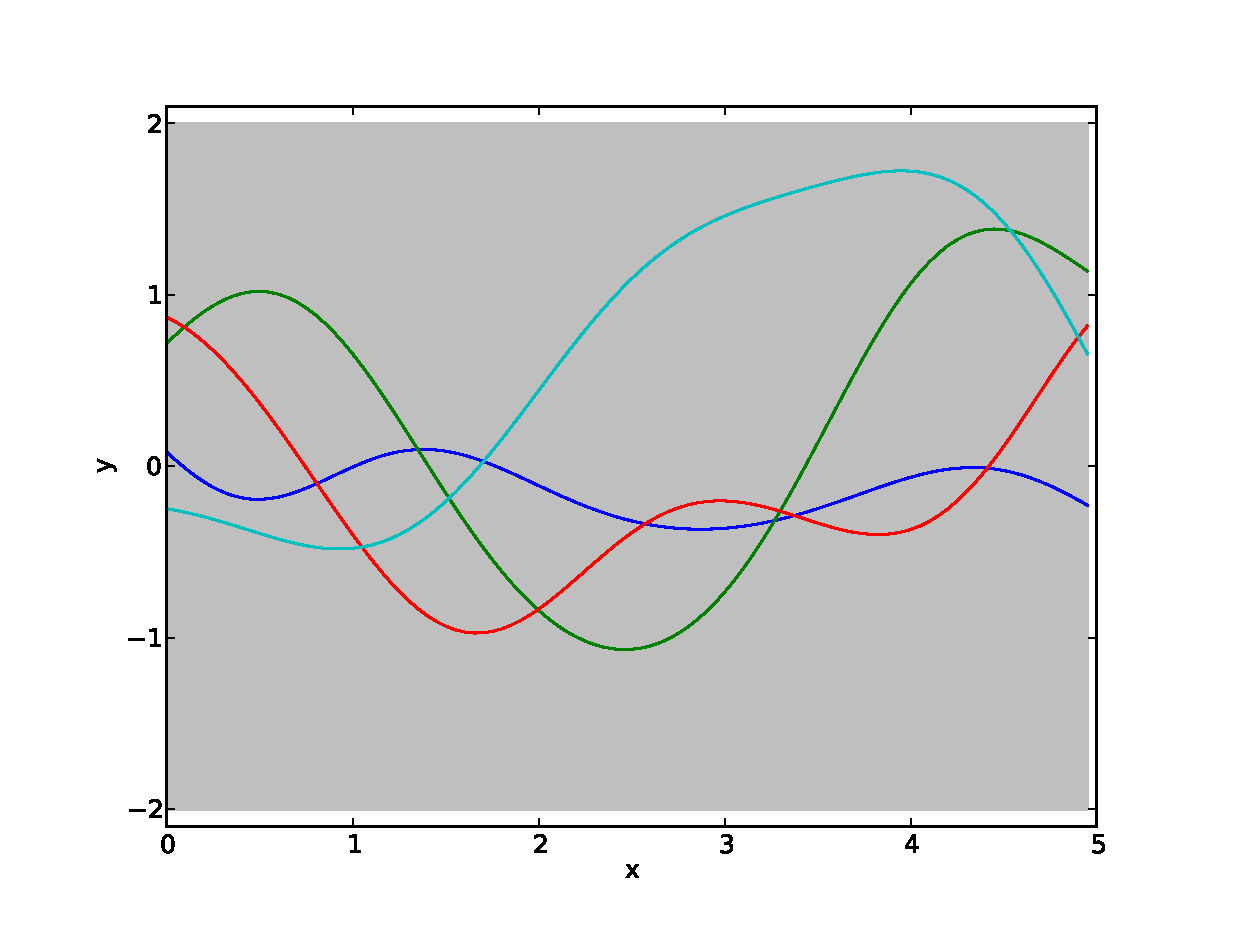
\includegraphics[width=0.49\textwidth]{fig3} 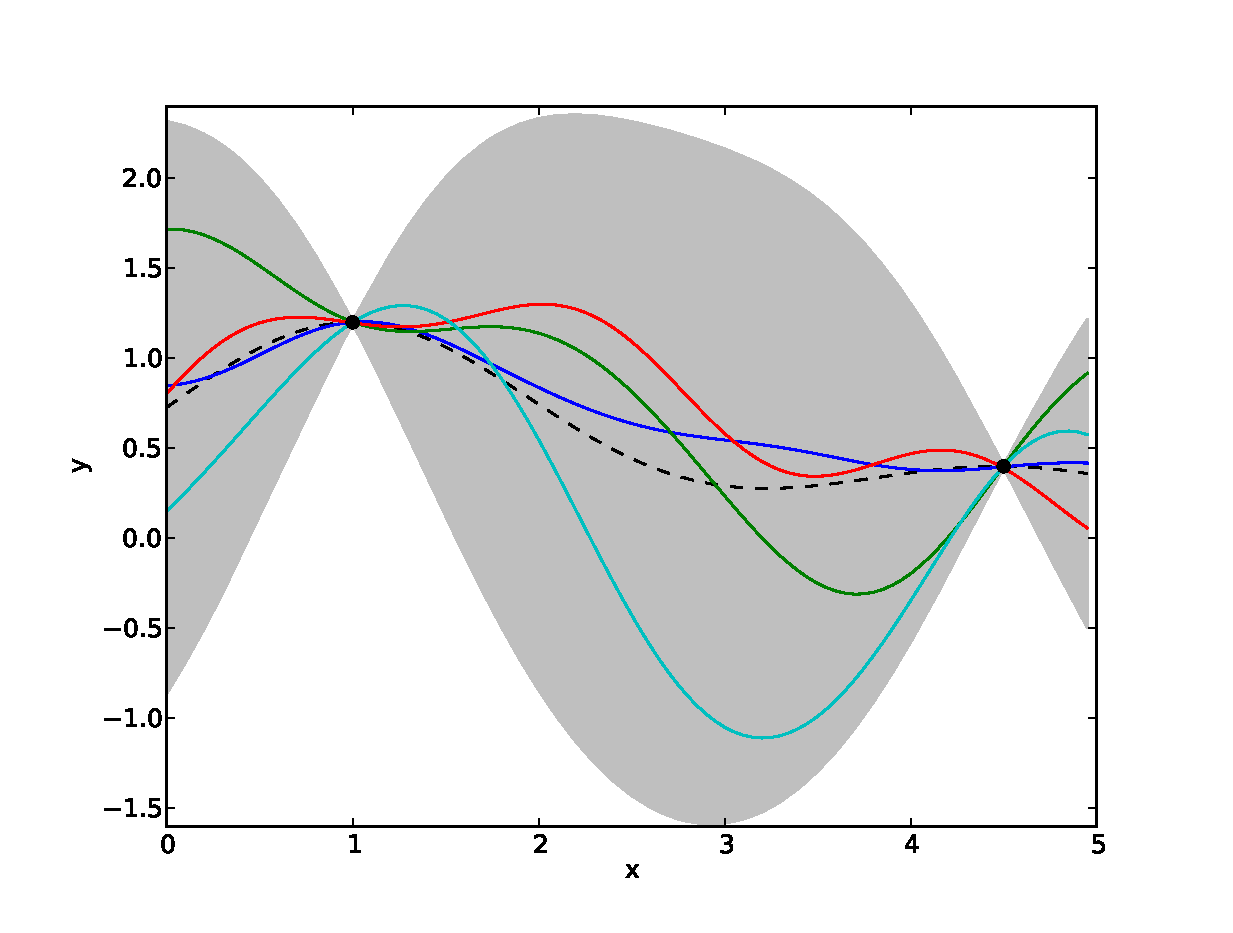
\includegraphics[width=0.49\textwidth]{fig4}
\caption{Left: Four samples drawn from the prior distribution \eqref{eq:prior}, using a covariance matrix generated from a Squared exponential covariance function \eqref{eq:se}. The shaded area gives the $2\sigma$ uncertainty of the prior distribution. Right: Same four samples this time drawn from the predictive distribution \eqref{eq:pred2}, conditioned on two noiseless data points (in the case of no noise GPR is essentially the same as the interpolation scheme known as \emph{Kriging} \cite[Chapter~3]{press2007}). The uncertainty is again $2\sigma$, and the dashed line gives the mean prediction.}
\label{fig:prediction}
\end{figure}

Adaptation of the hyperparameters can also be done through Bayes' Theorem:
%
\begin{equation}
p(\boldsymbol{\theta}|\mathbf{y},\mathbf{x},M_i) = \frac{p(\mathbf{y}|\mathbf{x},\boldsymbol{\theta},M_i)p(\boldsymbol{\theta}|M_i)}{p(\mathbf{y}|\mathbf{x},M_i)},
\label{eq:hyper}
\end{equation}
%
which gives the posterior of the hyperparameters, note that the likelihood for the hyperparameters is the same as the marginal likelihood in \eqref{eq:loglike}. In order to get the correct predictive description one multiply \eqref{eq:pred2} with the above equation~\eqref{eq:hyper} and marginalizes with respect to $\boldsymbol{\theta}$. This is the correct Bayesian way to adapt the hyperparameters -- unfortunately the integrals that appear here are not generally analytically tractable, and one has to resort to some kind of numerical integration scheme. Another way is to simply employ the classical approach and optimize the marginal likelihood in \eqref{eq:loglike} with respect to the hyperparameters. According to \cite{rasmussen2006} this is okay for the hyperparameters, since the location of the maximum likelihood is usually well localized in hyperparameter space. In this project we will employ the classical approach for the hyperparameters, using the downhill simplex algorithm built into scipy to do the optimization.

\chapter{Description of Software}
\label{sec:description}

In this section I'll describe how to use the software that was developed for this project. All code is contained in the files \pyt{covar.py} and \pyt{gp.py}. \pyt{covar.py} just contains a selection of covariance functions and a helper function used to calculate covariance matrices, while \pyt{gp.py} contains all the real code.

The main function in \pyt{gp.py} is simply called \func{gp}, and takes up to five arguments and one keyword argument. There are three ways to call \func{gp}:
%
\begin{quote}
\va{fprior},\va{fcovar} = \func{gp}(\va{hypdict},\va{covar},\va{x},\va{tol}=\dt{1e-5}) \\
\va{nlml}               = \func{gp}(\va{hypdict},\va{covar},\va{x},\va{y},\va{tol}=\dt{1e-5}) \\
\va{$\bar{\textup{f}}_\star$},\va{ferror},\va{fcovar},\va{$\alpha$},\va{nlml} = \func{gp}(\va{hypdict},\va{covar},\va{x},\va{y},\va{x$_\star$},\va{tol}=\dt{1e-5}).
\end{quote}
%
Going through the inputs, \va{hypdict} is a dictionary with the hyperparameters and will be discussed later. \va{covar} is the covariance function to be used (usually picked from \pyt{covar.py}). \va{x} is the training inputs, and \va{y} is the training targets. \va{x$_\star$} is the prediction inputs. \va{tol} is a keyword giving the tolerance of the solution, more about that later. If \func{gp} is called with three arguments it assumes that one wants to draw samples from the prior, and returns the predicted mean (which is always constant in my implementation), and covariance matrix for the GP -- this is used when one want to draw samples from the GP prior as we did in \fref{fig:prediction}. If \func{gp} is called with four inputs it assumes that one is training the GP and it only returns the \emph{negative log marginal likelihood} -- we use the negative value so that it works with the downhill simplex optimizer. Finally if \func{gp} is called with five arguments it assumes we're doing predictions and returns the mean estimate of the GP, the error estimate, the full covariance matrix, a parameter, \va{$\alpha$}, that is useful when working with composite covariance functions, and again the negative log marginal likelihood.

As mentioned above \va{hypdict} is a dictionary in which we give hyperparameters of the GP. It always has the format:
%
\begin{quote}
\va{hypdict} = \{\red{'hyp'}: \dt{list}, \red{'mean'}: \dt{float}, \red{'sigma'}: \dt{float}\}.
\end{quote}
%
\red{'hyp'} contains a list of the hyperparameters of the chosen covariance function, \red{'mean'} gives the mean value of the GP, which in my implementation has to be a constant value, while \red{'sigma'} gives the white noise component of the GP. The algorithm used for finding the mean prediction and covariance of the GP is identical to Algorithm~2.1 in~\cite[page~19]{rasmussen2006} and I won't reprint it here, and only describe the main points: Instead of computing the inverse of $K + \sigma_n^2 I$ directly, the algorithm uses the fact that covariance matrices are both \emph{symmetric} and \emph{positive definite}, and computes the \emph{Cholesky Decomposition} \cite{wiki:chol} for the covariance matrix. The algorithm then uses the Cholesky decomposition to solve several system of equations to get the desired results. The main reason for using the Cholesky Decomposition is that it according to~\cite{rasmussen2006} is more stable than straight matrix inversion. Some numerical instability however remains in the code, which is why I've introduced the the \va{tol} keyword. This simply adds a small value (default \dt{$10^{-5}$}) to the diagonal of the covariance matrix to do away with floating point errors that might otherwise make the Cholesky Decomposition impossible.

Another function inside \pyt{gp.py} is \func{draw\_sample} which is used to draw random samples from the GP. It can be called in either of two ways:
%
\begin{quote}
\va{sample} = \func{draw\_sample}(\va{hypdict},\va{covar},\va{x},\va{ns}=\dt{1},\va{seed}=\dt{None}) \\
\va{sample} = \func{draw\_sample}(\va{hypdict},\va{covar},\va{x},\va{y},\va{x$_\star$},\va{ns}=\dt{1},\va{seed}=\dt{None})
\end{quote}
%
The inputs are the same as for \func{gp} (in fact \func{draw\_sample} calls \func{gp} from inside), and depending on the number of inputs the samples are drawn from either a prior or conditioned GP. the \va{ns} keyword gives the number of samples drawn (default is \dt{1}), while the \va{seed} keyword determines the seed of the pseudo-random number generator (default is \dt{None}). Note that if \va{sigma} $\neq 0$ in the \va{hypdict} dictionary, a noisy sample will be drawn. We used \func{draw\_sample} to draw both the prior and conditioned samples in \fref{fig:prediction}.

The last function inside \pyt{gp.py} is \func{hyper\_optimize}, which as the name suggests tries to optimize the hyperparameters. It is called the following way:
%
\begin{quote}
\va{hypdict},\va{nlml} = \func{hyper\_optimize}(\va{hypdict0},\va{covar},\va{x},\va{y},\va{mask}).
\end{quote}
%
\va{hypdict0} is a dictionary of same form as \va{hypdict} containing the first guess of the values of the hyperparameters. \va{mask} is also a dictionary with the same form as \va{hypdict0}, but with values equal to \dt{True} or \dt{False} depending on whether one wishes to optimize this hyperparameter or not. An example would be:
%
\begin{quote}
\va{mask} = \{\red{'hyp'}: \dt{True}, \red{'mean'}: \dt{False}, \red{'sigma'}: \dt{True}\}.
\end{quote}
%
In this example \func{hyper\_optimize} would not try to optimize the mean of the GP. This masking property is useful if one don't want to optimize either \va{sigma} (as would be the case when doing interpolation) or \va{mean}. In the current version of the code one cannot single out single hyperparameters that one wishes not to optimize, it's all or none. \func{hyper\_optimize} uses the downhill simplex function, \func{scipy.optimize.fmin}, built into scipy which is not really optimal for the task. The reason for this is that matrix inversion is a $\mathcal{O}(n^3)$ task, and is carried out for every function call. A better approach would be a gradient optimizer which means that one will only have to invert the matrix once, hereby reducing the computational overhead. In an eventual future expansion of the code both the implementation of masking of individual hyperparameters, and optimization using a gradient method would have high priority.

\chapter{Tests}
\label{sec:tests}

In this section I'll go through some of the tests that I applied to check the validity of my code. All figures in this section as well as \fref{fig:regression} and~\ref{fig:prediction} were generated by running \pyt{figures.py}.

We've already seen a couple of tests of the code in \fref{fig:regression} and~\ref{fig:prediction}. In \fref{fig:regression} we drew six noisy samples from an underlying function chosen to be a 2nd order polynomial. Applying GPR to the problem using a squared exponential covariance function was seen to give good results. \fref{fig:prediction} was done by using \func{draw\_sample} to draw random samples from first the GP prior and afterwards the GP conditioned on two data points.

It is illustrative to see what would happen if we extend the range of the x-axis in \fref{fig:regression} to see what happens far away from the data. We do that in \fref{fig:test1}, which is completely equivalent to \fref{fig:regression} except for the wider range. It is seen that far away from the data the predictions fall back to the prior distribution. This is not strange taking into consideration that the data was modelled using a Squared Exponential covariance function, which only give high covariance when close to data points.

\begin{figure}[htb]
\centering
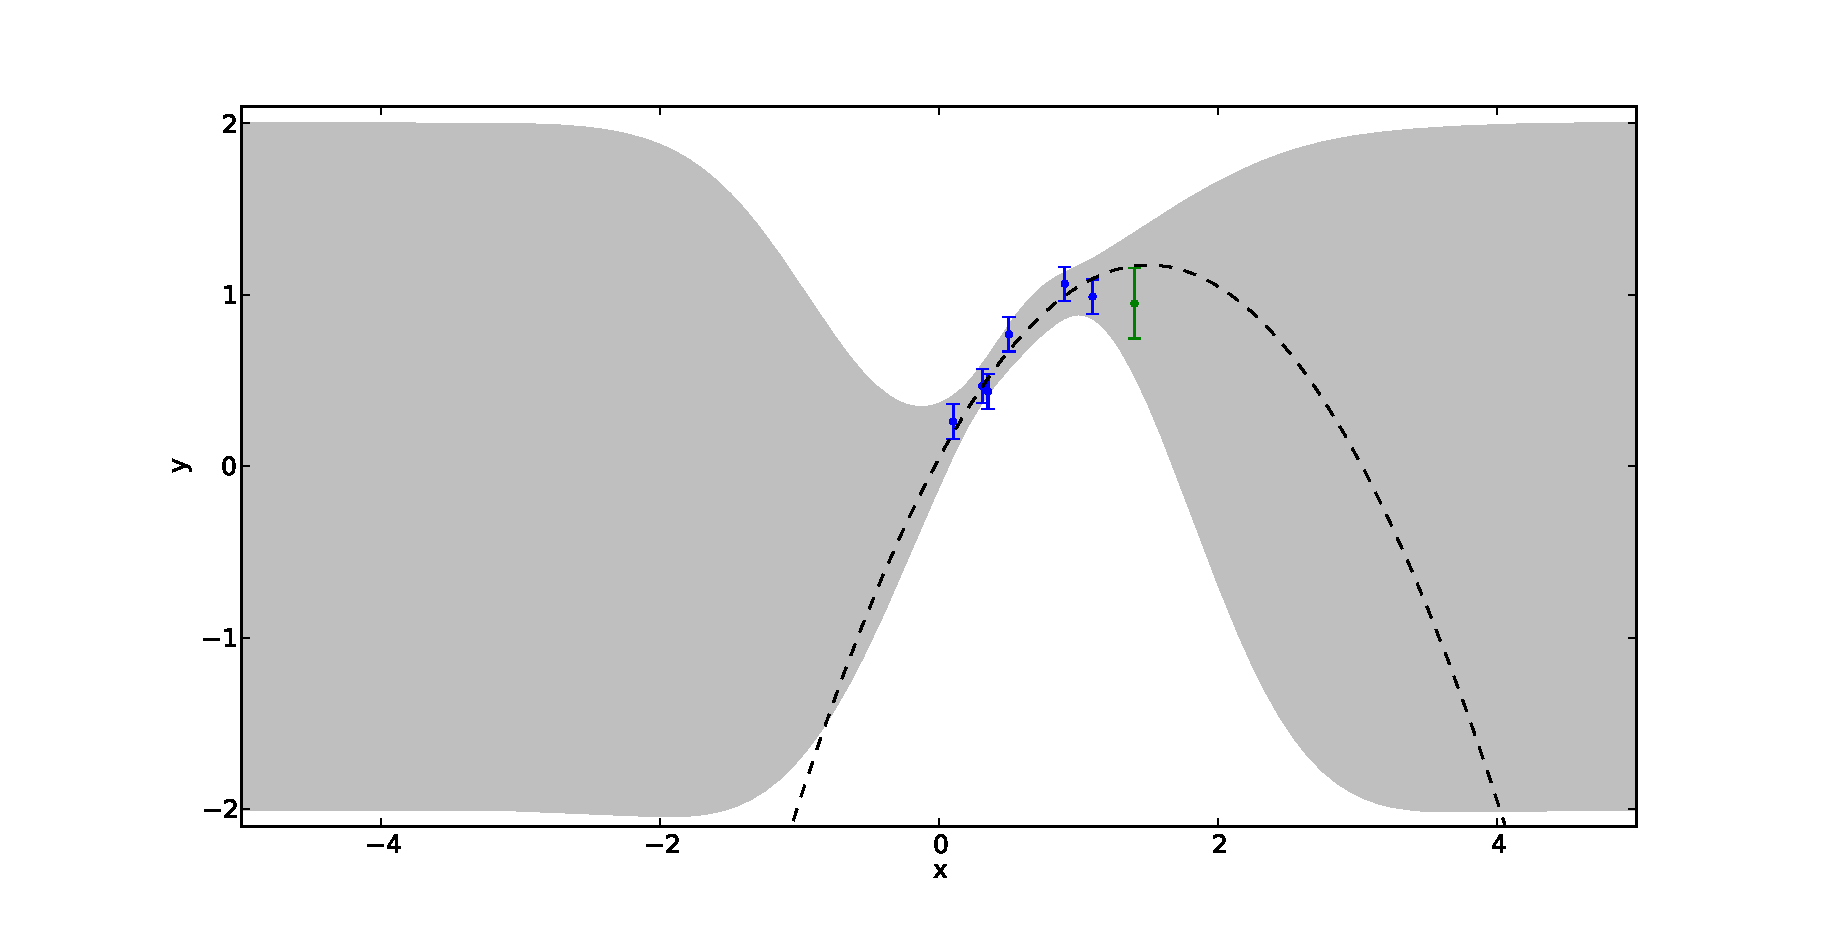
\includegraphics[width=\textwidth]{fig5}
\caption{Same as \fref{fig:regression}, but with wider range.}
\label{fig:test1}
\end{figure}

Another illustrative case to consider is what happens when one varies the hyperparameters. In \fref{fig:varyhyper} I've shown data generated from a GP with a squared exponential covariance function with hyperparameters $(\ell,\sigma_f,\sigma_n)=(1,1,0.1)$, along with the predictions. In the following two plots I've shown the predictions with hyperparamters being $(0.3,0.5,0.0005)$ and $(3,1,0.9)$ respectively. It's very clear to see that neither of the two latter cases describe the data as well, as the first one.

\begin{figure}[htb]
\centering
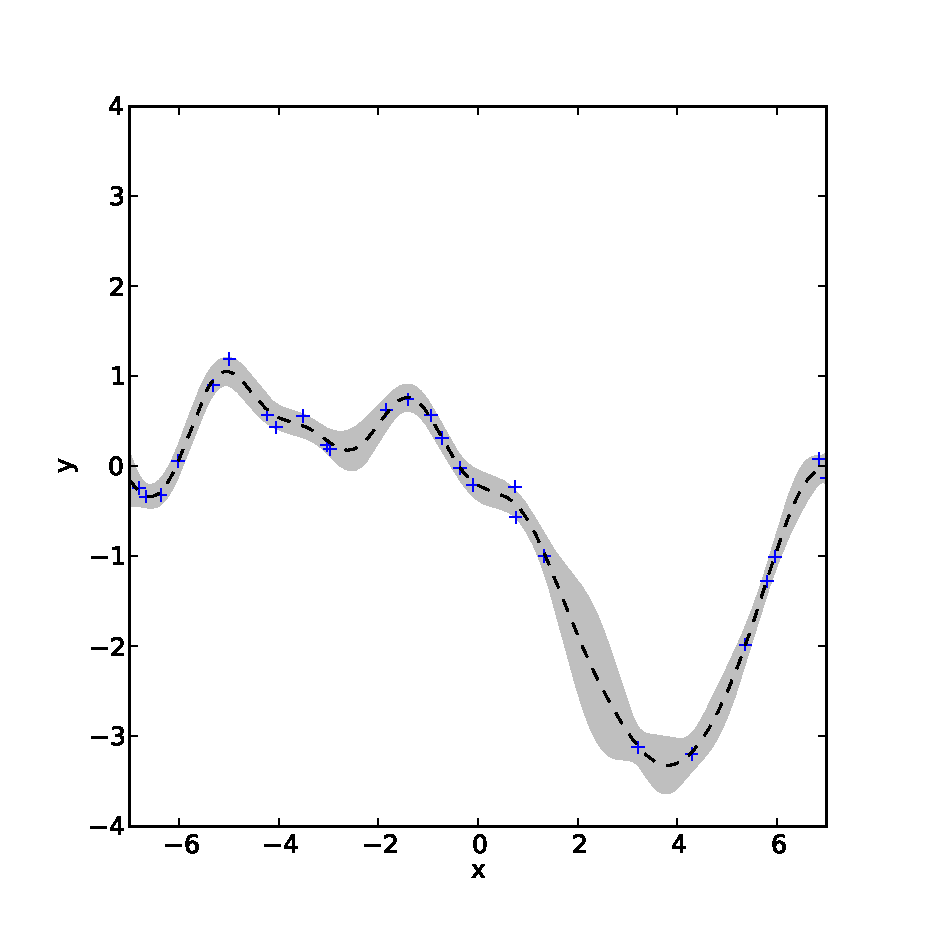
\includegraphics[width=0.49\textwidth]{fig6} \\ 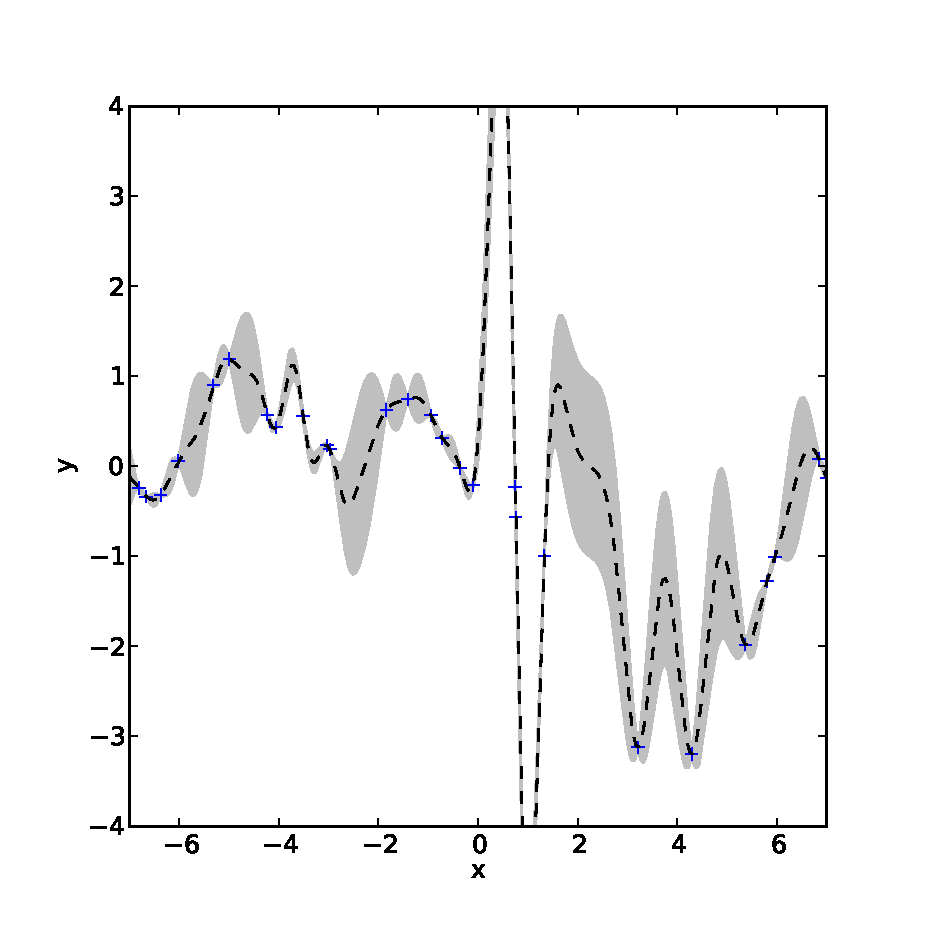
\includegraphics[width=0.49\textwidth]{fig7} 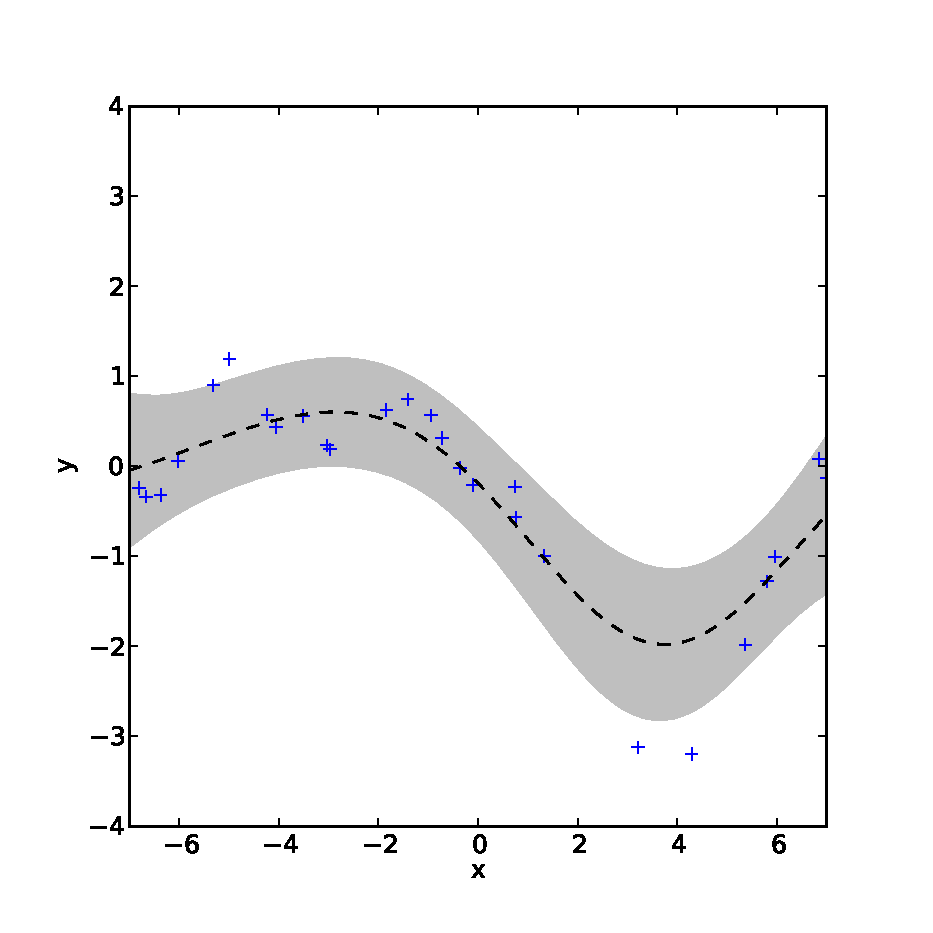
\includegraphics[width=0.49\textwidth]{fig8}
\caption{Top: Data drawn from a GP with hyperparameters $(\ell,\sigma_f,\sigma_n)=(1,1,0.1)$, and predictions using the same hyperparameters. Bottom Left: Same data but predictions using hyperparameters $(0.3,0.5,0.0005)$. Bottom Right: Same data but predictions using hyperparamters $(3,1,0.9)$}
\label{fig:varyhyper}
\end{figure}

By using the property that sums and products of covariance functions are themselves valid covariance functions \cite[Chapter~4]{rasmussen2006}, one can create composite covariance functions for data that cannot be described well by a single covariance function. An example of this is shown in \fref{fig:composite} where we have observations consisting of an oscillatory signal with a rising trend. We choose to model this with a sum between a squared exponential covariance function \eqref{eq:se} and a periodic covariance function:
%
\begin{equation}
k(x,x') =  \sigma_f^2 \exp \left(- \frac{2\sin^2 \left( \pi \frac{x-x'}{P} \right)}{\ell^2} \right).
\label{eq:per}
\end{equation}
%
The periodic covariance function gives peaks of high covariance with a period, $P$. $\ell$ is a smoothness hyperparameter that determine the ``intermediate'' covariance in between the periodic covariance peaks, while $\sigma_f$ as in the case of the Squared Exponential covariance function determines the overall scale. All the hyperparameters for this covariance function are scale parameters.

\begin{figure}[htb]
\centering
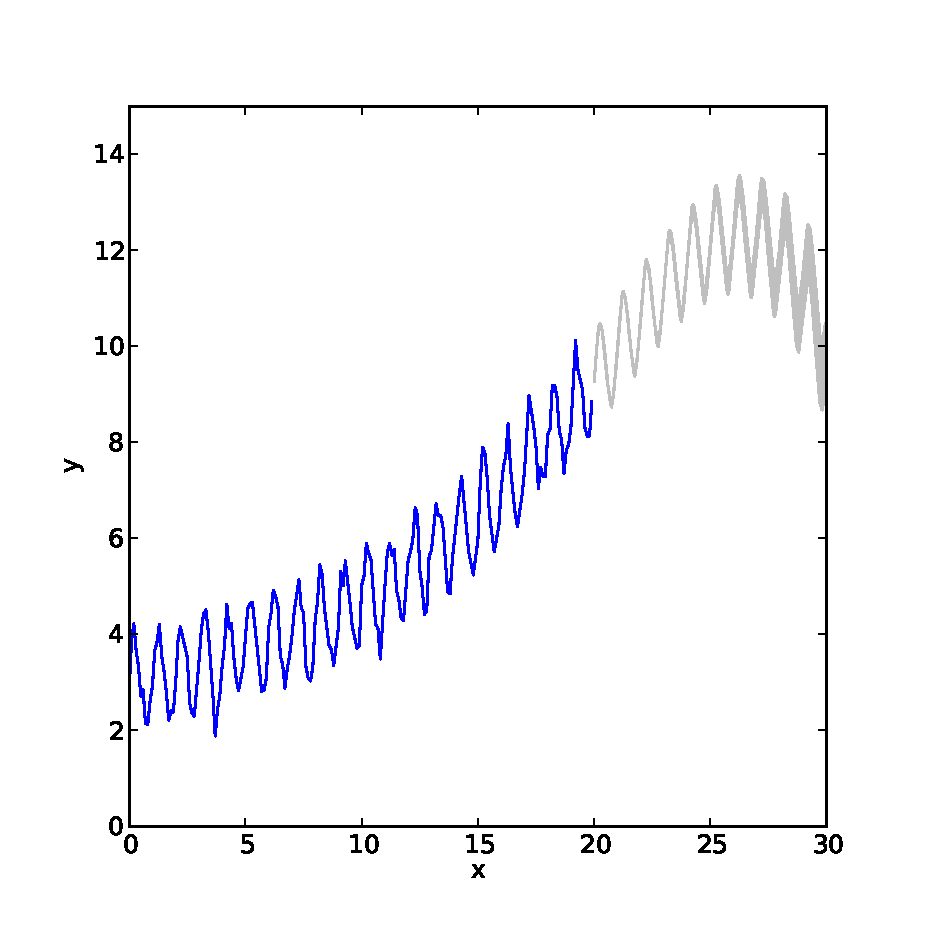
\includegraphics[width=0.49\textwidth]{fig9} 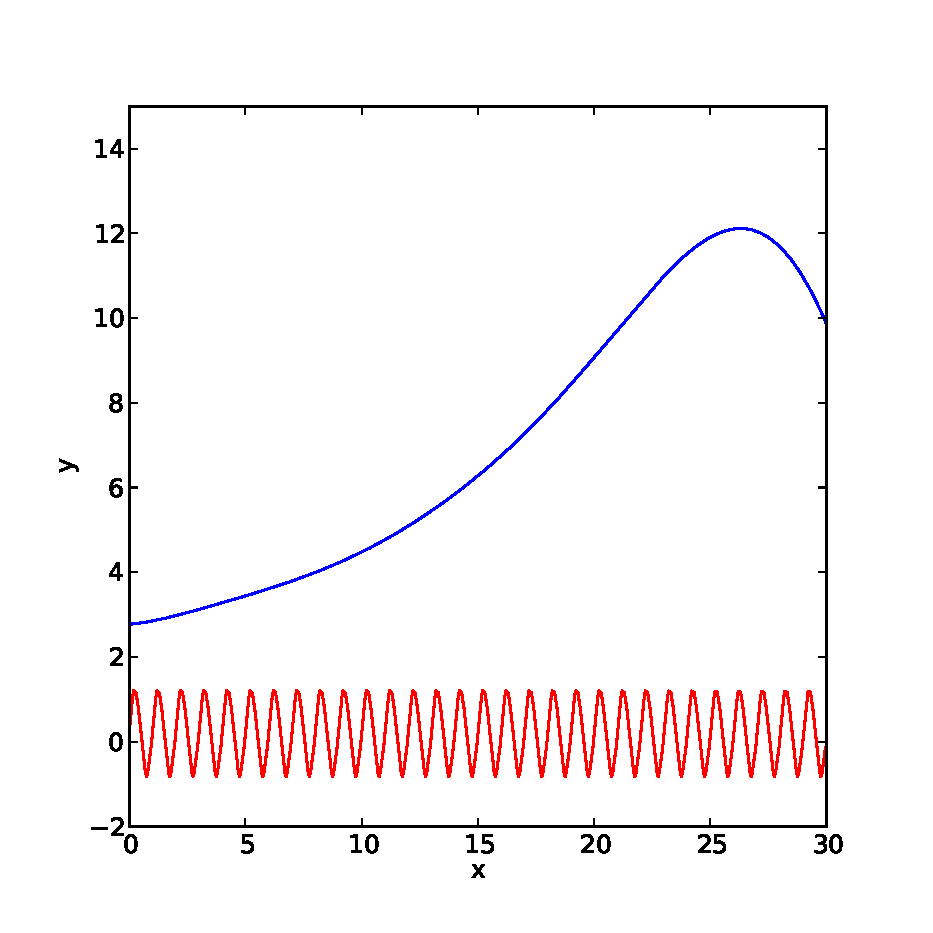
\includegraphics[width=0.49\textwidth]{fig10}
\caption{Left: The data and predictions ahead in time. Looking at the data the predictions looks reasonable for a while until they start dropping although there's nothing in the data to suggest this. Right: Predictions of the Squared Exponential, and periodic term.}
\label{fig:composite}
\end{figure}

The composite covariance function then ends up having the appearance:
\begin{equation}
k(x,x') = \theta_1^2 \exp\left( -\frac{(x-x')^2}{2\theta_2^2}\right) + \theta_3^2 \exp \left(- \frac{2\sin^2 \left( \pi \frac{x-x'}{\theta_4} \right)}{\theta_5^2} \right) + \sigma_n\delta_{x,x'}, \nonumber
\end{equation}
where I've included the noise hyperparameter in the function for clarity. Running the above covariance function though \func{hyper\_optimize} gives the result $(\theta_1,\theta_2,\theta_3,\theta_4,\theta_5,\sigma_n)=(3.66,12.25,1.00,0.51,1.27,0.21)$. The log marginal likelihood for the model is $-5.39$. Note that the predictions initially look very good but that they begin to drop after a short while, although there's no indication of this in the data. This is simply where GPR hits it's limit -- if we believed that the trend would continue to go up, we should choose another way to model this than the Squared Exponential covariance function, since this guarantees nothing of the sort. This example simply goes to show that you should always be careful when interpreting model results, no matter how they were created.

When you have a composite covariance function that can be described as a sum of several distinct covariance functions it's worth noting that the predictions for the distinct terms of the covariance function can be calculated. Recall from \eqref{eq:pred2} that the mean prediction of the latent function, $\mathbf{f}_\star$ can be written:
\begin{equation}
\bar{\mathbf{f}}_\star = K_\star^T\left[K + \sigma_n^2 I \right]^{-1}(\mathbf{y}-\mathbf{m}). \nonumber
\end{equation}
Say that your covariance function can be written as a sum of two other covariance functions so that $k = k_1 + k_2$. Then it's possible to expand the above equation:
\begin{align}
\bar{\mathbf{f}}_\star &= \left(K_{\star,1}^T + K_{\star,2}^T\right)\left[K_1 + K_2 + \sigma_n^2 I \right]^{-1}(\mathbf{y}-\mathbf{m}) \nonumber \\
 &= K_{\star,1}^T\left[K_1 + K_2 + \sigma_n^2 I \right]^{-1}(\mathbf{y}-\mathbf{m}) + K_{\star,2}^T\left[K_1 + K_2 + \sigma_n^2 I \right]^{-1}(\mathbf{y}-\mathbf{m}), \nonumber
\end{align}
%
where the first term will be the predictions belonging to $k_1$, and the second term the predictions belonging to $k_2$. We show this property to the right in \fref{fig:composite}, where the blue line is the mean predictions of the Squared Exponential covariance function, and the red line is the mean predictions of the periodic covariance function.

\chapter{Example: Measurements of tide height}
\label{sec:example}

The GPR procedure is applied to a real data consisting on measurements of tide height in Southern England. The data is freely available from \url{http://www.sotonmet.co.uk/}, and I downloaded all available data from July 2011. The resulting time series which can be seen in \fref{fig:tideheight} has lots of holes in it. This is because of network outages and periods where the sensor gets stuck. I've removed bad points due to the sensor being stuck beforehand. The goal of the procedure is so find a good covariance function for the data, optimize the hyperparameters and see if we can predict the tide height on points with no data available.



\chapter{Discussion \& Conclusion}
\label{sec:discussion}

Over the course of this project a lot of the subtleties of GPR has become clear to me. In this section I'll try to follow up on what I've learned along the way. If the goal of the GPR is to do interpolation 

\bibliographystyle{plain}
\bibliography{cit.bib}

\end{document}
